\documentclass[12pt]{article}

\fontfamily{lmss}
\usepackage{fullpage}
\usepackage{amsmath}
\usepackage{amsthm}
\usepackage{url}
\usepackage{multicol}
\usepackage{enumerate}
\usepackage{graphicx}
\usepackage{color}

\usepackage{xcolor}

\usepackage{tikz}
\usetikzlibrary{graphs}
\usetikzlibrary{arrows.meta,shapes,shapes.geometric}
\usetikzlibrary{positioning, quotes}

\tikzset{
  % Two node styles for game trees: solid and hollow
  solid node/.style={circle,draw,inner sep=1.2,fill=black},
  hollow node/.style={circle,draw,inner sep=1.2},
  % styles for long branch labels
  left label/.style={above left,midway},
  right label/.style={above right,midway}
}

\usepackage{hyperref}
\hypersetup{
    colorlinks=true,
    linkcolor=blue,
    filecolor=magenta,      
    urlcolor=blue,
}

\usepackage{geometry}
\geometry{
  top=1in,            % <-- you want to adjust this
  bottom=1in,
  left=1in,
  right=1in,
  headheight=3ex,       % <-- and this
  headsep=4ex,          % <-- and this
}

\usepackage{lastpage}
\usepackage{fancyhdr}
\pagestyle{fancy}
\fancyhf{}
\renewcommand{\footrulewidth}{0.4pt}
\lhead{CS 486/686}
\rfoot{Page \thepage\ of \pageref{LastPage}}

\setlength{\parskip}{\baselineskip}%
\setlength{\parindent}{0pt}%

\usepackage{tcolorbox}
\tcbuselibrary{breakable}
\newenvironment{markscheme}
{
    \renewcommand{\parskip}{\baselineskip}
    \begin{tcolorbox}[
        colback=blue!10,
        colframe=blue!10,
        sharp corners,
        breakable
    ]
    \textbf{Marking Scheme:}
}
{
    \end{tcolorbox}
}

\newenvironment{sol}
{
    \renewcommand{\parskip}{\baselineskip}
    \begin{tcolorbox}[
        colback=magenta!10,
        colframe=magenta!10,
        sharp corners,
        breakable
    ]
    \textbf{Solutions:}
}
{
    \end{tcolorbox}
}


\lhead{CS 486/686}
\chead{Spring 2021}
\rhead{Assignment 2}
\cfoot{v1.0}
\lfoot{\copyright Alice Gao 2021}

\title{CS 486/686 Assignment 2 (128 marks)}
\author{Alice Gao}
\date{Due Date: 11:59 pm ET on Wednesday, June 30, 2021}

\begin{document}

\maketitle

% \section*{Changes}

% \begin{itemize}
% \item v1.1
% \end{itemize}

\newpage
\section*{Academic Integrity Statement}

{\color{red} If your written submission on Learn does not include this academic integrity statement with your signature (typed name), we will deduct 5 marks from your final assignment mark.}


I declare the following statements to be true:

\begin{itemize}
\item 
The work I submit here is entirely my own.

\item 	
I have not shared and will not share any of my code with anyone at any point. 

\item 
I have not posted and will not post my code on any public or private forum or website.

\item 	
I have not discussed and will not discuss the contents of this assessment with anyone at any point.

\item 
I have not posted and will not post the contents of this assessment and its solutions on any public or private forum or website. 

\item 
I will not search for assessment solutions online.

\item 
I am aware that misconduct related to assessments can result in significant penalties, possibly including failure in the course and suspension. This is covered in Policy 71: https://uwaterloo.ca/secretariat/policies-procedures-guidelines/policy-71.
\end{itemize}

By typing or writing my full legal name below, I confirm that I have read and understood the academic integrity statement above.


\newpage
\section*{Instructions}

\begin{itemize}
\item
Submit any written solutions in a file named \verb+writeup.pdf+ to the A1 Dropbox on \verb+Learn+. Submit any code to \verb+Marmoset+ at \url{https://marmoset.student.cs.uwaterloo.ca/}. 
No late assignment will be accepted. This assignment is to be done individually.

\item 
I strongly encourage you to complete your write-up in Latex, using this source file. If you do, in your submission, please replace the author with your name and student number. Please also remove the due date, the Instructions section, and the Learning goals section. Thanks!

\item
Lead TAs: 
\begin{itemize}
\item
Dake Zhang (dake.zhang@uwaterloo.ca)
\item 
Ethan Ward (e7ward@uwaterloo.ca)
\end{itemize}
The TAs' office hours will be posted on MS Teams.
\end{itemize}

\section*{Learning goals}
%
{\bf Constraint Satisfaction Problem}
\begin{itemize}
\item
Formulate a given problem as a constraint satisfaction problem. Define the variables, the domains, and the constraints.
\item
Trace the execution of the AC-3 arc consistency algorithm on a given CSP.
\end{itemize}

{\bf Decision Trees}
\begin{itemize}
\item 
Implement the decision tree learner algorithm to learn a decision tree using a data set with real-valued features.
\item
Determine the prediction accuracy of a decision tree on a data-set.
\item
Perform pre-pruning and post-pruning. Determine the best parameter value for pruning using cross validation.
\end{itemize}




\newpage
\section{Wooden Stick Grid Puzzle (38 marks)}

We have a 4 by 4 grid and 16 wooden sticks of 4 different lengths. The possible lengths are 1, 2, 3, and, 4. There are 4 wooden sticks of each length. Our goal is to place the wooden sticks vertically on the grid while satisfying the following constraints:
\begin{itemize}

\item (All Different Constraints) In each row, the lengths of the sticks are all different. In each column, the length of the sticks are all different.
    
\item (Viewing Constraints) There is a number on each side of a row or a column. This number describes the exact number of different sticks that a person can see if the person views the sticks from that side of the row or column. (This is a 3D puzzle.)
    
See Figure~\ref{fig:stick_puzzle_example} for an example. 
The number on the left side of a row is $2$ and the number on the right is $3$. [2 4 3 1] is a valid placement for this row. From the left, a person can see the sticks 2 and 4. From the right, a person can see the sticks 1, 3, and 4. 
    
\begin{figure}[ht!]
    \centering
    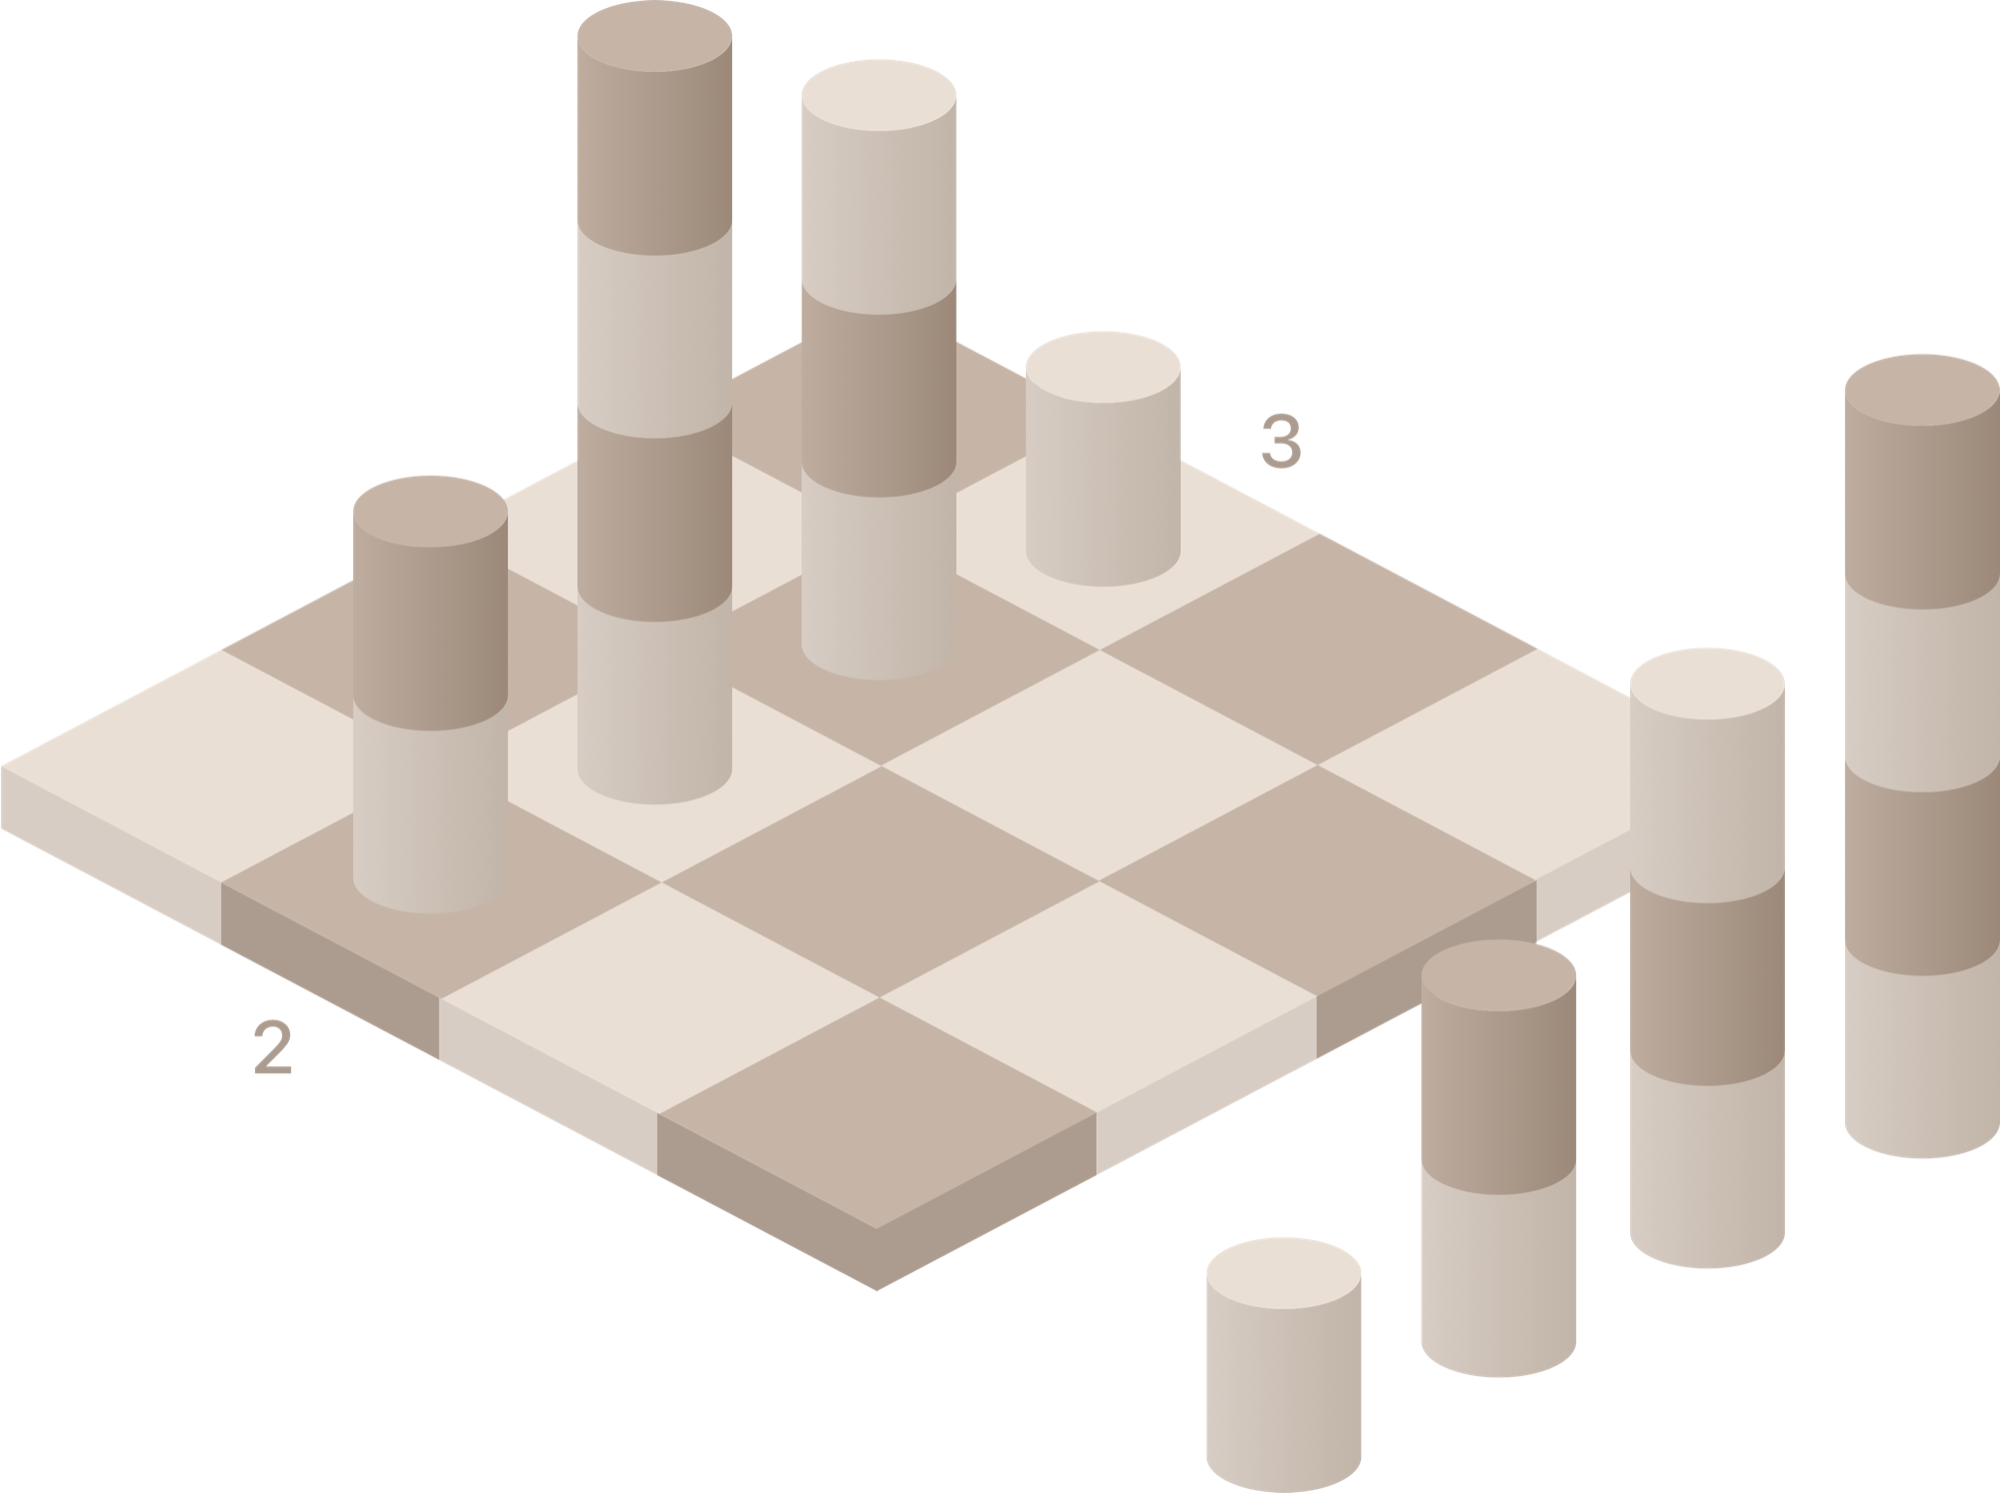
\includegraphics[scale=0.15]{images_posted/stick_puzzle.png}
    \caption{Stick puzzle example}
    \label{fig:stick_puzzle_example}
\end{figure}

    
\end{itemize}

Complete the following tasks using Table~\ref{tab:wood-stick}.

\begin{table}[ht!]
\centering
\begin{tabular}{c|c|c|c|c|c}
  & 2 & 3 & 3 & 1 &   \\ \hline
2 &   &   &   &   & 1 \\ \hline 
1 &   &   &   &   & 3 \\ \hline 
3 &   &   &   &   & 2 \\ \hline 
2 &   &   &   &   & 2 \\ \hline 
  & 3 & 1 & 2 & 2 &  \\ 
\end{tabular}
\caption{Wooden Stick Grid Puzzle Example 1}
\label{tab:wood-stick}
\end{table}

\begin{enumerate}[(a)]

\item 
\label{csp_1}
Solve the puzzle in Table~\ref{tab:wood-stick} by hand. Submit the final answer. 

\begin{markscheme}
(2 marks) Correct solution.
\end{markscheme}
    
    


\item 
Formulate the puzzle in Table~\ref{tab:wood-stick} as a constraint satisfaction problem. We have provided the variable definitions below. Describe the domains of the variables and the constraints. Feel free to use words or mathematical expressions. 

{\bf Variables: }

A variable represents the sequence of four numbers from left to right in a row or the sequence of four numbers from top to bottom in a column. 

Let $R_i$ denotes the variable for the $i$-th row from the top. $i \in \{1, 2, 3, 4\}$ $R_1$ denotes the top row. 

Let $C_j$ denotes the variable for the $j$-th column from the left. $j \in \{1, 2, 3, 4\}$. $C_1$ denotes the leftmost column.

\begin{markscheme}
(8 marks)

\begin{itemize}
    \item (2 marks) Domains
    \item (6 marks) Constraints
\end{itemize}

\end{markscheme}


\item 
Consider the puzzle in Table~\ref{tab:wood-stick}.

For each unary constraint on a variable, remove all the values in the variable's domain that violate the unary constraint. Afterwards, write down the updated domains of all the variables. 

\begin{itemize}
\item $R_1 \in \{$ 
\item $R_2 \in \{$ 
\item $R_3 \in \{$ 
\item $R_4 \in \{$ 
\item $C_1 \in \{$
\item $C_2 \in \{$
\item $C_3 \in \{$
\item $C_4 \in \{$
\end{itemize}

\begin{markscheme}
(8 marks)

\begin{itemize}
    \item (4 marks) The domains for $R_1 \dots R_4$.
    \item (4 marks) The domains for $C_1 \dots C_4$.
\end{itemize}

\end{markscheme}


\item
Start with the reduced domains of the variables from the previous part. We will continue solving the puzzle using the AC-3 arc consistency algorithm.

Execute the AC-3 algorithm on the puzzle for 8 steps as described below. 

For each step, we have provided the arc to be removed from the set $S$. list the values removed from the domain of the variable and whether we need to add any arcs back to S. We have completed step 1 as an example.

After the 9 steps, indicate whether the algorithm should terminate or not. If the algorithm should terminate, describe the outcome of the algorithm execution.

\begin{enumerate}[(1)]
\item Remove $\langle R_3, (R_3, C_1) \rangle$ from $S$.

Remove 1243, 1342 from the domain of $R_3$.

Add nothing back to $S$.

\item Remove $\langle R_4, (R_4, C_1) \rangle$ from $S$.
\item Remove $\langle C_1, (R_1, C_1) \rangle$ from $S$.
\item Remove $\langle R_4, (R_4, C_1) \rangle$ from $S$.
\item Remove $\langle C_4, (R_3, C_4) \rangle$ from $S$.
\item Remove $\langle C_3, (R_4, C_3) \rangle$ from $S$.
\item Remove $\langle C_2, (R_3, C_2) \rangle$ from $S$.
\item Remove $\langle R_2, (R_2, C_2) \rangle$ from $S$.
\item Remove $\langle R_1, (R_1, C_3) \rangle$ from $S$.
\end{enumerate}

\begin{markscheme}
(18 marks)

\begin{itemize}
    \item (2 marks) for each of the 8 steps.
    \item (2 marks) for the result after 8 steps.
\end{itemize}
\end{markscheme}


\item
We tackled the same problem with two methods: (1) solving it by hand, and (2) solving it by executing the AC-3 algorithm. How are these two approaches similar or different? Discuss your observations and thoughts in a few sentences.

\begin{markscheme}

(2 marks) provide a reasonable discussion.

\end{markscheme}


\end{enumerate}



\newpage
\section{Decision Trees (90 marks)}
\label{question_dt}

You will implement an algorithm to build a decision tree for a Yeast data-set. Read more about the data set  \href{https://archive.ics.uci.edu/ml/datasets/Yeast}{here}.

The data-set has real-valued features. When generating a decision tree, use {\bf a binary split} at each node. At each node in the decision tree, choose a feature and a split point for the feature using the expected information gain metric, and the node should test whether a feature has a value greater than the split point or not. Along a path from the root node to a leaf node, we may test a real-valued feature multiple times with different split points.

{\bf Information on the provided code}

We have provided several files below.
\begin{itemize}

\item \verb+data.csv+ includes the data set. \verb+dt_global.py+ defines several useful global variables. \verb+dt_provided.py+ defines some useful functions for reading the data-set and splitting the data-set into different folds.

Do not modify these files and do not submit these files.

\item \verb+dt_core.py+ contains empty functions for generating the tree and performing pruning. \verb+dt_cv.py+ contains empty functions for performing cross validation. You need to complete all the empty functions in these files.

\end{itemize}

{\bf The Attributes in an Anytree Node}

We use the \verb+anytree+ package to store the decision tree. Our unit tests make use of several custom attributes in an \href{https://anytree.readthedocs.io/en/latest/api/anytree.node.html#anytree.node.node.Node}{Anytree Node}. Make sure that you use these attributes so that you will pass our tests.

\begin{itemize}

\item \verb+name+: string. Each Node requires the \verb+name+ attribute. The \verb+name+ of each node should be unique.  You can generate this attribute in any way you like. We won't test this attribute.
% Otherwise, the plot of the tree will merge nodes that have the same \verb+name+s.

\item \verb+parent+: Node. To construct the tree properly, you either need to set a Node's \verb+parent+ attribute or a Node's \verb+children+ attributes. See \href{https://anytree.readthedocs.io/en/latest/api/anytree.node.html}{the Node documentation} for more details. We recommend setting the \verb+parent+ attribute of each Node. Once the \verb+parent+ attribute is set, the \verb+children+ attribute will be set automatically by Anytree. If you set the left child node's parent attribute before setting the right child node's parent attribute, then you can retrieve the left child node as \verb+children[0]+ and the right child node as \verb+children[1]+.

\item The \verb+feature+ attribute stores the chosen feature as a string. The \verb+split+ attribute stores the split point value as a float. Any non-leaf node should have the \verb+feature+ and \verb+split+ attributes.

\item The \verb+decision+ attribute stores the decision as an integer. Any leaf node should have the \verb+decision+ attribute.

\end{itemize}

{\bf Tie-Breaking Rules}

Please use the following tie-breaking rules to ensure that your program passes the unit tests.
\begin{enumerate}[(1)]
\item 
If a leaf node has examples with different labels, we need to determine a decision using majority vote. If there is a tie, return the label with the smallest value. For example, if a leaf node has two examples with label $4$ and two examples with label $5$, the majority decision should be $4$.

\item
Given a feature, if there are multiple split points with the same maximum information gain, choose the split point with the smallest value. For example, suppose that, the split points \verb+9.3+ and \verb+9.5+ tie for the maximum information gain among all the spilt points for the feature, we will choose to split on \verb+9.3+.

\item
Suppose that, for each feature, we have identified the split point with the maximum information gain. Given the best split points for the features, if multiple split points have the same maximum information gain, choose the first feature based on the order of the features in the first row of the \verb+data.csv+ file. The order is given below.

\verb+mcg, gvh, alm, mit, erl, pox, vac, nuc+.

For example, suppose that the information gain for the best split point for \verb+mcg+ and the best split point for \verb+pox+ tie for the maximum information gain (among the best split points for all the features), we will choose to split on the best split point for \verb+mcg+.

\end{enumerate}

{\bf Ten-Fold Cross-Validation}

The purpose of performing cross validation is to choose the best value for a parameter. We will use cross validation to choose the best parameter value in pre-pruning and post-pruning. 

In ten-fold cross-validation, each data point serves double duty --- as training data and validation data. 
\begin{enumerate}

\item 
Split the data into $10$ subsets using \verb+preprocess+ in \verb+dt_provided.py+.

\item 
For each parameter value, perform ten rounds of learning. In the $i$-th round, the validation set is the $i$-th fold and the training set consists of the remaining $9$ folds.

\item 
In the $i$-th round, learn a decision tree with the parameter value using the training set. Determine the prediction accuracy of the decision tree on the training set and on the validation set. The prediction accuracy is the fraction of examples that the tree predicts correctly. (Don't worry if you generate different trees in different rounds. We do not care about the trees generated. We only care about the prediction accuracies.)

\item 
After the ten rounds, calculate the average prediction accuracy of the decision tree on the training set and on the validation set, where the average is taken over the ten rounds. For each parameter value, you will produce two numbers, the average prediction accuracy on the training set and the average accuracy on the validation set. 
 
\item 
Choose the parameter value with the highest average prediction accuracy on the validation set. 
\end{enumerate}

{\bf Packages: }

You can assume that all the packages below are available in our testing environment. If you want to use a different package, please post a question on Piazza.
%
\begin{itemize}
\item numpy (version 1.19.5)
\item anytree (version 2.8.0)
% \item graphviz (version 0.16)
% \item matplotlib (version 3.3.4)
\end{itemize}


{\bf Efficiency: }

The unit tests will evaluate your implementation for correctness and efficiency. If your implementation does not terminate within a pre-defined time limit, it will fail the unit test. We set the time limits by taking our run-times and multiplying it by a small constant factor. For your information, our program terminates within 1 second for part b1, within 20 seconds for part b2, and within 10 seconds for part b3.

Here are some advice for improving your program efficiency. 
\begin{itemize}
\item Limit the external packages that your program uses. Do not use \verb+pandas+ --- it will slow down your program considerably. Limit your use of \verb+numpy+. It's sufficient to use arrays and dictionaries only.

\item Think hard about how to perform pruning efficiently. You may be able to performing pruning without modifying the tree. You may also be able to start with a previously generated tree instead of building a full tree all over again.
\end{itemize}

{\bf Please complete the following tasks.}

\begin{enumerate}[(a)]
\item 
Complete all the empty functions in \verb+dt_core.py+ and \verb+dt_cv.py+ and submit both files on Marmoset. 

\begin{markscheme}
(85 marks)

\begin{itemize}

% \verb+dt_core.py+

\item \verb+get_splits+ \\
(1 public test + 4 secret tests) * 2 marks = 10 marks

\item \verb+choose_feature_split+ \\
(1 public test + 4 secret tests) * 3 marks = 15 marks

\item \verb+split_examples+ \\
(1 public test + 4 secret tests) * 1 mark = 5 marks

\item \verb+learn_dt+ (and \verb+split_node+)

1 public test * 1 mark 
+ 2 simple secret tests * 2 marks 
+ 2 full-tree secret tests * 5 marks 
= 1 + 4 + 10 = 15 marks

\item \verb+predict+ \\
(1 public test + 4 secret tests) * 1 mark = 5 marks

\item \verb+get_prediction_accuracy+ \\
(1 public test + 4 secret tests) * 1 mark = 5 marks

\item \verb+post_prune+ \\
(1 public test + 4 secret tests) * 2 marks = 10 marks

% \verb+dt_cv.py+
\item \verb+cv_pre_prune+ \\
(1 public test + 4 secret tests) * 2 mark = 10 marks 

\item \verb+cv_post_prune+ \\
(1 public test + 4 secret tests) * 2 mark = 10 marks

\end{itemize}

\end{markscheme}

\item 
Complete the questions below. Include your answers in \verb+writeup.pdf+ and submit it on Learn.

\begin{enumerate}[(1)]
\item 
Suppose that we built a decision tree called \verb+tree-full+ using the data set. What is the maximum depth of \verb+tree-full+? 
% on the data-set using the decision tree learner algorithm discussed in lectures 6 and 7. For each real-valued feature, use the procedure described in lecture 7 slide 44 to choose a split point for the feature.

\begin{markscheme}

(1 mark) Correct value of the maximum depth of the tree.
\end{markscheme}


\item 
Suppose that we want to pre-prune \verb+tree-full+ using the maximum depth criterion and using majority voting to make decisions at leaf nodes. What is the best value of the tree's maximum depth through ten-fold cross-validation? Please use the range $[0, 30]$ for the maximum depth.

\begin{markscheme}

(1 mark) Correct value of the best maximum depth for pre-pruning.
\end{markscheme}


\item 
Suppose that we want to post-prune \verb+tree-full+ using the minimum number of examples criterion.

For post-pruning, grow a full tree first. Define a value for the minimum number of examples. Next, keep track of all the nodes that only has leaf nodes as its descendants. Let's call these nodes \verb+leaf parents+. For each \verb+leaf parent+ node, if the number of examples at the node is less than the pre-defined value, then delete its children and convert this node to a leaf node with majority decision. \verb+Repeat+ this process until the number of examples at every \verb+leaf parent+ node is greater than or equal to the pre-defined value.

What is the best value for the minimum number of examples  through ten-fold cross-validation? Use the range $[0, 300]$ with an increment of $20$ for the minimum number of examples.

\begin{markscheme}

(1 mark) Correct value of the best minimum number of examples for post-pruning.
\end{markscheme}


\item 
In the previous parts, you have experimented with several ways of building a decision tree for the data-set. If you had a choice, what is the best strategy you can use to generate a decision tree for this data-set? You can choose one of the strategies in this assignment or you can think of any other strategies. 

Explain your strategy and justify why it is your best choice.
\begin{markscheme}

(2 marks) A reasonable explanation
\end{markscheme}


\end{enumerate}

\end{enumerate}

\end{document}





























